% This file was converted to LaTeX by Writer2LaTeX ver. 1.4
% see http://writer2latex.sourceforge.net for more info
\documentclass[a4paper]{article}
%\usepackage[latin1]{inputenc}
\usepackage[T1]{fontenc}
\usepackage[english]{babel}
\usepackage{amsmath}
\usepackage{amssymb,amsfonts,textcomp}
\usepackage{color}
\usepackage{xcolor,colortbl}
\usepackage{sectsty}
\usepackage{tocloft}
\usepackage{fancyhdr}
\usepackage{afterpage}
\fancyhf{}
\usepackage{lastpage}
\usepackage{datetime}
\usepackage{colortbl}
\usepackage{array}
%\usepackage[top=0.7882in,bottom=0.4917in,left=1.25in,right=1.25in,nohead,includefoot,foot=0.5083in,footskip=0.97720003in]{geometry}
\usepackage[headheight=110pt]{geometry}
%\usepackage{supertabular}
\usepackage{hhline}
\usepackage{caption}
\usepackage{hyperref}

\usepackage{graphicx}
\usepackage{verbatim}
\pagestyle{fancy}
%\usepackage{titlesec}
\afterpage{\cfoot{\thepage}}

%new packages & rules
\linespread{1.1} % Definition of the linespread
%\usepackage[square,sort,comma,numbers]{natbib}
\usepackage{amsmath}
\usepackage{amssymb}
\mathchardef\mhyphen="2D % Define a "math hyphen" 
\usepackage{amsthm}
\usepackage{amsmath}
\usepackage{amsfonts}
\usepackage{amssymb}
\usepackage{amsthm}


\usepackage[utf8]{inputenc}
\usepackage[english]{babel}
\usepackage{amsthm}
\theoremstyle{definition}
\newtheorem{definition}{Definition}
\newtheorem{example}{Example}


%\usepackage{eufrak}
\newcommand{\R}{\mathbb{R}}
\newcommand{\N}{\mathbb{N}}
\usepackage[ruled,vlined,noend]{algorithm2e}
\usepackage{natbib}
\usepackage{pgf}
\usepackage{tikz}
\usetikzlibrary{arrows,automata}
% to start new page for each new section
%\titlespacing*{\section}
%{0pt}{6.5ex plus 1ex }{6.3ex plus .2ex}
%\titlespacing*{\subsection}
%{0pt}{6.5ex plus 1ex }{6.3ex plus .2ex}

%\allsectionsfont{\centering}
\setlength{\headsep}{0.2in}

%\newdateformat{bkdate}{\twodigit{\THEDAY}-\twodigit{\THEMONTH}-\twodigit{\THEYEAR}}
%\dmyydate


\definecolor{datacroninner}{rgb}{0.0,0.0,0.5647059}
\newcommand{\datacroncolor}{\color{datacroninner}}
\chapterfont{\datacroncolor}  % sets colour of chapters
\sectionfont{\datacroncolor}  % sets colour of sections
\subsectionfont{\datacroncolor}  % sets colour of sections
\subsubsectionfont{\datacroncolor}
\hypersetup{colorlinks=true, linkcolor=datacroninner, citecolor=datacroninner, filecolor=datacroninner, urlcolor=blue}

\newcommand{\documenttitle}{\ Master Thesis Proposal}
%\newcommand{\horizongeneral}{\ H2020-ICT-2015 \dmyydate \today}
%\lhead{
\includegraphics[width=122pt]{figures/datACRONDXYTemplate201512162-img001.png}}
\chead{\documenttitle}
%\rhead{\horizongeneral}
\lfoot{}
\fancyfoot[C]{Page \thepage \hspace{1pt}}
%\cfoot{Page \thepage \hspace{1pt} of \pageref{LastPage}}

\cfoot{Page \thepage}
\rfoot{}


%\makeatletter
\newcommand\arraybslash{\let\\\@arraycr}
%\makeatother
% Footnote rule
\setlength{\skip\footins}{0.0469in}
\renewcommand\footnoterule{\vspace*{-0.0071in}\setlength\leftskip{0pt}\setlength\rightskip{0pt plus 1fil}\noindent\textcolor{black}{\rule{0.0\columnwidth}{0.0071in}}\vspace*{0.0398in}}
\setlength\tabcolsep{1mm}
\renewcommand\arraystretch{1.3}
\newcounter{Table}
\renewcommand\theTable{\arabic{Table}}

\title{\documenttitle}
\author{Ehab Qadah \\\\Supervisor:
	PD Dr. Michael Mock}
\date{\dmyydate \today}
\begin{document}
\pagestyle{fancy}
\newcommand{\sectionbreak}{
\clearpage{\pagestyle{fancy}}}

\pagenumbering{gobble}

%\cfttoctitlefont{\datacroncolor}
%

%\title{\Huge Grant Agreement No: 687591}
%{\centering
%\par}
%\clearpage{\pagestyle{fancy}}
%%\setcounter{page}{1}
%\maketitle{\Huge}
%%\centering
%\title{\Large \textbf{ Predicting patterns of moving objects based
%	on contextual information with distributed online learning \\ 
%Distributed Online Learning for Forecasting Patterns of Moving Objects Events Streams \\
%Distributed Online Learning for Forecasting Patterns in Event Streams of Moving Objects}}
%{\centering
%\Large
%\par}
%\maketitle

%{\centering
%
\includegraphics[width=2.5835in,height=0.6634in]{figures/datACRONDXYTemplate201512162-img001.png}
% \par}






%\begin{flushleft}
%\centering
%\begin{tabular}{lm{5.83516in}l}
%\hline
%%\centering
%\title{\documenttitle}
%\maketitle
%\\\hline
%\end{tabular}
%\end{flushleft}





%\begin{flushleft}
%\begin{tabular}{|m{0.25\textwidth}|m{0.75\textwidth}|}
%%\multicolumn{2}{|m{5.8350596in}|}{Deliverable Form}\\\hline
%\rowcolor{datacroninner}
%{\bfseries\color{white}Deliverable Form}& \\\hline
%Project Reference No. &
%H2020-ICT-2015 687591\\\hline
%Deliverable No.  & 8.1\\\hline
%Relevant Work Package: & WP 8\\\hline
%Nature: &R\\\hline
%Dissemination Level: &PU\\\hline
%Document version: &1.0\\\hline
%Due Date: &29/02/2016\\\hline
%Date of latest revision: &16/12/2015\\\hline
%Completion Date: &~\\\hline
%Lead partner: &UPRC\\\hline
%Authors: &
%George Vouros\\\hline
%Reviewers: &~\\\hline
%Document description: &
%This deliverable documents the main project procedures. These procedures have been presented and agreed at the kickoff
%
%meeting chaired by the coordinator.\\\hline
%Document location: &
%Desktop/Projects/datACRON/Project/Dels\\\hline
%\end{tabular}
%\end{flushleft}

%\clearpage

%\section*{HISTORY OF CHANGES}
%\thispagestyle{empty}
%\addcontentsline{toc}{section}{HISTORY OF CHANGES}
%\begin{flushleft}
%\begin{tabular}{|m{1.10in}|m{1.10in}|m{1.10in}|m{1.10in}|m{1.10in}|}
%\hline
%\rowcolor{datacroninner}
%{\bfseries\color{white} Version} &{\bfseries\color{white} Date} & {\bfseries\color{white} Changes} & {\bfseries\color{white} Author} & {\bfseries\color{white} Remarks}\\\hline
%~ &~ &~ &~ &~\\\hline
%\end{tabular}
%\end{flushleft}

%\clearpage

%\section*{EXECUTIVE SUMMARY}
%\addcontentsline{toc}{section}{EXECUTIVE SUMMARY}
%%\clearpage


%\section*{TABLE OF CONTENTS}
%\addcontentsline{toc}{section}{TABLE OF CONTENTS}
%
%
%
%\setcounter{tocdepth}{3}
%\renewcommand\contentsname{}
%\renewcommand{\cfttoctitlefont}{\datacroncolor}
%\tableofcontents
%\section*{TERMS \& ABBREVIATIONS}
%\addcontentsline{toc}{section}{TERMS \& ABBREVIATIONS}
%
%\section*{LIST OF FIGURES}
%\addcontentsline{toc}{section}{LIST OF FIGURES}
%%\cftloftitlefont{\datacroncolor}
%\listoffigures
%\section*{LIST OF TABLES}
%\addcontentsline{toc}{section}{LIST OF TABLES}
%
%\listoftables

\begin{titlepage}
		\begin{center}
			% 
\includegraphics[scale=0.1]{img/logo}\\[1cm]
			\setlength{\tabcolsep}{0pt}
			\begin{tabular}{>{\raggedleft}m{2.5cm}>{\centering}m{\dimexpr\textwidth - 5cm\relax}>{\raggedright}m{2.5cm}}
				
\includegraphics[width=\linewidth]{chapters/figures/logo.pdf}%
				&%
				\textbf{\large } \\[5pt]%
				\textbf{\large}%
				&%
				
\includegraphics[width=\linewidth]{chapters/figures/iais.pdf} %
			\end{tabular}
			
			
			\textsc{\LARGE Rheinische\\[5mm] Friedrich-Wilhelms-Universität Bonn}\\[1.0cm]
			
			\textsc{\Large Mathematisch-naturwissenschaftliche fakultät}\\[1.0cm]
			
			\textsc{\Large Master Thesis Proposal }\\[1.5cm]
			
			% Title
			{ \Large \bfseries 
%				Predicting patterns of moving objects based
%				on contextual information with distributed online learning \\ 
%				Distributed Online Learning for Forecasting Patterns of Moving Objects Events Streams \\
				Distributed Online Learning for Large-scale  \\Pattern Prediction over Real-time Event Streams}\\[2.9cm]
			
			% Author and supervisor
			\begin{minipage}[t]{0.4\textwidth}
				\begin{flushleft} \large
					\emph{Author:}\\
					Ehab \textsc{Qadah}
				\end{flushleft}
			\end{minipage}
			\begin{minipage}[t]{0.5\textwidth}
				\begin{flushright} \large
					\emph{First Examiner:} \\
					PD.~Dr.~Michael~\textsc{Mock} \\[0.5cm]
					\emph{Second Examiner:} \\
					Prof.~Dr.~Stefan \textsc{Wrobel} \\[0.5cm]
					
					%\emph{Abteilung:} \\
					%Autonome Intelligente Systeme
				\end{flushright}
			\end{minipage}
			
			\vfill
			
			% Bottom of the page
			{\large  \hspace{1cm} \date{\dmyyyydate \today} }
			
		\end{center}
	\end{titlepage}
\clearpage

\section*{Abstract}

Predicting full matches of complex patterns from various real-time event streams is an important utility for the decision maker in many application domains such as maritime surveillance, financial services, and sensor networks. Such a utility allows him/her to proactively react to the new situations and enhances the operational decision making. An event stream is an unbounded collection of timely ordered data observations in the form of an attribute tuple that is composed of a value from finite event types along with other categorical and numerical features. For example, in the context of maritime surveillance, patterns prediction over real-time tracking streams of moving vessels is useful to alert maritime operation mangers about suspicious activities (e.g., fast sailing vessels near ports) before they happen, in this scenario, the event stream of a moving vessel consists of spatial-temporal and kinematic information along with the vessel's identification and its trajectory related event types. However, processing real-time streaming data is challenging since data streams are large in nature and continuously keep on coming at a high rate. 
% we describe the design and implementation of a system called% 
\par To this end, in this thesis, we present an online, distributed and scalable patterns prediction system over massive input event streams. The proposed approach is based on a novel approach that combines the  distributed online prediction protocol \citep{kamp2014communication} with the event forecasting with Pattern Markov Chain system\citep{alevizos2017event}, in order to provide an online and large-scale patterns prediction system over distributed real-time event streams. 

 \par We leverage an existing online probabilistic forecasting model, which consists of the event forecasting with Pattern Markov Chain~\citep{alevizos2017event}. This system gives the ability to predicate when a pattern within a stream of events will be fully matched. In addition, we integrate the distributed online synchronization protocol \citep{kamp2014communication} to provide distributed online learning capabilities between the prediction models in a communication-efficient manner. This protocol enables us to dynamically synchronize the distributed local prediction models of the multiple input event streams.
 
  In some practical applications the input event streams may belong to different distributions, we propose to divide the input event streams into similar groups, in order to combine the corresponding predictions models to construct a representative global model in each group. The aggregation operation refers to the synchronization operation (e.g., joint average of the local models) in the distributed online learning protocol, which is performed by a central coordinator that constructs and distributes a global prediction model for the input event streams based on the  local models. In addition, we are using one of the modern Big Data frameworks for stream processing i.e., Apache Flink \footnote{\url{https://flink.apache.org/}} to implement the proposed system.
\par We aim to provide an architecture and implementation of a system for large-scale patterns prediction over multiple input event streams. Our approach exploits the collaborative learning from multiple input streams by combing their associated predication models in a dynamic way. 
 
\par We will analysis and develop the proposed approach, and evaluate the effectiveness through empirical experiments over synthetic event streams and real-word data streams of moving objects, in particular, events streams related to trajectories of moving vessels, which are provided in the context of the datAcron project\footnote{\url{http://www.datacron-project.eu/}}.

%Furthermore, we will try to provide probabilistic guarantees for the new proposed %method by performing theoretical analysis procedures. 


{\large\textbf{\\ \\ Acknowledgment\\\\}}
This work is supported by the EU H2020 datAcron project (grant agreement No 6875).

{\large\textbf{\\ Keywords\\\\}}
Big Event Data Streams, Stream processing,Large-scale Patterns Prediction, Maritime Surveillance, Apache Flink, Distributed Pattern Markov Chain\\


\pagenumbering{arabic}
\setcounter{page}{1}
\thispagestyle{fancy}
\chapter{Introduction}


\section{Motivation}
\par In the past decade, technological advancements have led to a growing availability of massive amounts of continuous event streams in many application domains such as social networks \cite{reuter2012event,mathioudakis2010twittermonitor}, Internet of Things (IoT) \cite{miorandi2012internet}, user activities on the web \cite{banerjee2001clickstream,metwally2005duplicate} and maritime monitoring \cite{patroumpas2015event,laxhammar2010conformal}.

\par These event streams used to be stored and processed later, while monitoring and processing them in real-time increases their value \cite{carney2002monitoring}. Moreover, the real-time streams provide the opportunity to implement reactive components within these domains.  For example, the ability to detect and predict the full matches of a pattern of interest (e.g., a certain sequence of events), defined by a domain expert, is typically important for operational decision-making tasks in their respective domains.

\par An event stream is an unbounded sequence of time-ordered data observations in the form of a tuple of attributes that is composed of a value from finite event types along with other categorical and numerical attributes \cite{agrawal2008efficient,schultz2009distributed,zhou_pattern_2015,flouris2017issues}. Event patterns (i.e., composite events of interest) are defined using a pattern language such as SQL-like \cite{schultz2009distributed} or regular expressions \cite{alevizos2017event}.

\par As an illustrative example, consider the event streams of a group of moving vessels in the context of maritime surveillance. The event stream of a moving vessel consists of spatio-temporal and kinematic information along with the vessel's identification and its trajectory related events, based on the Automatic Identification System (\ac{ais}) \cite{ais} messages that are continuously sent by the vessel. Hence, leveraging event patterns prediction over real-time streams of moving vessels is useful to alert maritime operation managers about suspicious activities (e.g., fast sailing vessels near ports or illegal fishing) before they happen \cite{patroumpas2015event}. 

\par However, processing the real-time streaming data poses new challenges, since the data streams are large, distributed in nature and continuously arrive at a high rate \cite{Babcock2002,Flouris2017}. To deal with these data streams in a fast and efficient manner, a distributed stream processing framework \cite{Spark,Flink,Storm} is usually used to implement the stream processing and analytic applications. 


\section{Thesis Overview}
% we describe the design and implementation of a system called% 
\par In this thesis, we present the design, implementation, and evaluation of a scalable and distributed system that provides online pattern prediction over multiple real-time streams of events. The proposed approach is based on a novel method that combines a distributed online learning protocol \cite{kamp2014communication} with online probabilistic prediction models based on pattern Markov chain technique \cite{alevizos2017event}. The underlying model provides online predictions about when a pattern is expected to be completed within each event stream, where the patterns are defined in the form of regular expressions over the event types in the stream.

\par In particular, we consider the setting when there are \emph{$K$} input event streams, and for each one of these streams, a local prediction model is built on a distinct node. As a result, \emph{$K$} models are maintained separately on \emph{$K$} distributed predictor nodes each of which is consuming a single event stream.


 \par We propose to make the predictors of the event streams collectively learn a global model in a distributed and communication-efficient fashion. We adapt the distributed online learning protocol \cite{kamp2014communication}, where the pattern predictors \cite{alevizos2017event} send their local models to a coordinator node. We introduce a new synchronization operator that combines these independent local models to create a stronger global model and share it among all the predictors.
  

\par In addition, we  implement our system on top of the Big Data framework for distributed stream processing Apache Flink \cite{Flink}, and the streaming platform Apache Kafka \cite{Kafka}. We also evaluate our proposed system over synthetic event streams, and large-scale real-world data streams related to movement events of vessels, which are provided in the context of the datAcron project\footnote{\url{http://www.datacron-project.eu/}}.

In summary, the main contributions of this thesis are the following:

\begin{itemize}

	\item  A new method of combining a distributed online learning protocol \cite{kamp2016communication} with pattern Markov chain predictors \cite{alevizos2017event} over multiple input event streams. It is based on enabling the collaborative learning and information exchange among the predictors in a communication-efficient manner.  
	
	\item A study of the characteristics of the proposed method, by providing a theoretical analysis of the synchronization operation within the distributed online learning protocol, in which it is provided a probabilistic guarantee of the learning efficiency. 
	
	\item The description of the scalable and distributed architecture for the proposed system for event patterns prediction over massive event streams, along with the building blocks for the system's workflow processing. The implementation details of the system on top of Apache Flink and Apache Kafka are also presented. 
	%The implementation is open
	%source9 source code: http:.....
	
	\item An extensive empirical evaluation of the proposed approach over real-world and synthetic streams of events.
  
\end{itemize}


\section{Publication}

Parts of this thesis have been published in \cite{Qadah}:\\ \\
\bibentry{Qadah}.

\section{Outline }

%\par The rest of this thesis is structured as follows. Chapter  provides a review  of the related work and used frameworks. In Chapter ~\ref{chapter:system}, we describe the problem of events pattern prediction, and our approach along with its practical and theoretical aspects.
% Chapter ~\ref{chapter:overview} presents how the proposed system was built, its architecture,  and the implementation details in Flink and Kafka.
% Chapter ~\ref{chapter:evaluation} presents the experimental setup and results of our system over event streams of moving vessels and synthetic event streams. Finally, we give the overall conclusions of this thesis, and we discuss some potential future directions in Chapter ~\ref{chap:conclusions}.
	
\par The rest of this thesis is organized as follows:\\
\\
\textbf{Chapter~\ref{chap:realred_work}} provides an overview of the related work on pattern prediction over event streams, and the distributed online learning techniques. It also gives an introduction to Apache Flink and Apache Kafka.
\\
\\
\textbf{Chapter~\ref{chapter:system}} describes the problem of pattern prediction over a single event stream and introduces the used base model based on event forecasting with pattern Markov chains method \cite{alevizos2017event}. It also presents our method for pattern prediction over multiple input event streams by leveraging the distributed online learning protocol \cite{kamp2014communication}. Additionally, it provides the theoretical analysis and a probabilistic learning guarantee of the proposed approach.  
\\
\\
\textbf{Chapter~\ref{chapter:overview}}  presents the architecture of the proposed system, and the implementation details in Flink and Kafka.
\\
\\
In \textbf{Chapter~\ref{chapter:evaluation}}, the experiments and results over real-world event streams of moving vessels and synthetic event streams are presented.
\\
\\
Finally, conclusions are given in \textbf{Chapter~\ref{chap:conclusions}}, along with potential directions for future work.



%We discuss the related work and used frameworks in Section ~\ref{sec:realred_work}. In Section ~\ref{sec:system}, we describe the problem of pattern prediction, our proposed approach, and the architecture of our system. The implementation details on top of Flink are presented in Section ~\ref{sec:impl} and the experimental results in Section ~\ref{sec:results}. We conclude in Section ~\ref{sec:concl}.



%List of paper to check: 
%1) Distributed Complex Event Processing with Query Rewriting (intro,def)


\chapter{Related Work and Background}
\label{chap:realred_work}


\par In this chapter, we survey some of the related research in the areas of pattern prediction over event streams task, and techniques of distributed online learning over data streams. We also give a brief overview of the Big Data technologies that we used to implement our proposed system.  
\section{Related work}


\subsection{Pattern Prediction over Event Streams}

\par Several approaches have been proposed to formalize the task of event patterns (complex events) prediction over time-evolving data streams.  One common way to formalize this task is to assume that the stream is a time-series of numerical values, and the goal is to predict at each time point $t$ the next observations at some future points $t+1$, $t+2$, etc., (or even the output of some function of future values)~\cite{montgomery_introduction_2015}. 


%The task of forecasting over time-evolving streams of data can be formulated in various ways and with varying assumptions.
%One common way to formalize this task is to assume that the stream is a time-series of numerical values, and the goal is to forecast at each time point $n$ the values at some future points $n+1$, $n+2$, etc., (or even the output of some function of future values). 
% This is the task of time-series forecasting ~\citet{montgomery_introduction_2015}.

\par Another way to formalize the prediction task is to view streams as sequences of events,
i.e., tuples of multiple attributes, such as \textit{id}, \textit{event type}, \textit{timestamp}, etc., and the goal is to predict future events or  patterns of events. In this work, we focus on the latter definition of forecasting (prediction of complex event patterns).  

\par A relevant work of the detection of event patterns task has been established in the field of temporal pattern mining. Where events are defined as 2-tuples of the form \((\mathit{EventType}, \mathit{Timestamp})\). The goal is to extract patterns of events in the form of association rules \cite{agrawal_mining_1993} or frequent episode rules \cite{mannila_discovery_1997}. 

\par These rule-based methods have been extended in order to be able to learn rules for predicting event patterns. For instance, in \cite{vilalta_predicting_2002}, an association rule mining technique is introduced. This technique works as following. Firstly, it extracts sets of event types that frequently lead to a target event (i.e., a rare event) within a time window of a fixed size. Then, it uses them to build a rule-based prediction model. Also,  ~\citet{weiss1998learning} proposed another rule-based method to predict rare events in a stream, using a genetic algorithm to find all predictive patterns to form prediction rules.  


\par On the other hand, ~\citet{laxman_stream_2008} have proposed a probabilistic model for calculating the probability of the immediately next event in the stream. Which is achieved by combining each frequent episode \cite{mannila1997discovery} that presents a partially-ordered set of event types with a Hidden Markov Model (HMM). In addition, ~\citet{fahed_efficient_2014} have proposed episode rules mining algorithm which predicts distant events by generating a set of episode rules in the form \(P \rightarrow Q \) where $P$ and $Q$ are two episodes. These rules have a minimal antecedent (in number of events) and temporally distant consequent.

\par In \cite{zhou_pattern_2015} a mining method is presented that finds the frequent sequential patterns in a stream of events, which are then used to generate prediction rules. The event stream is processed into batches, in each batch the events are consumed to find the prefix matches from the discovered frequent patterns, to predict future events using different strategies of prediction scoring.

% add more details about the cep
\par Event pattern prediction has also attracted some attention from the field of complex event processing (\ac{cep}), where the CEP system consumes a stream of low-level events to detect patterns of events (composite events) that are defined using pattern-based languages, these languages provide logic, sequence, and iteration operators such as SQL-like languages \cite{Cugola:2012:PFI:2187671.2187677}. 
\par One such early approach is presented in \cite{muthusamy_predictive_2010}, which is based on converting the complex event patterns to automata, and subsequently, Markov chains are used in order to estimate when a pattern is expected to be fully matched. 
%TODO: add more details%
\par Moreover, ~\citet{alevizos2017event} have recently presented a similar approach based on the pattern Markov chain (\ac{pmc}), where the PMC model is employed in order to provide future time intervals during which a full match of the pattern is expected with a probability above a confidence threshold. In this thesis, we leverage this method as the base prediction model for each input event stream (see Section ~\ref{sec:Event-Forecasting-PMC}). 

\subsection{Distributed Online Learning}

\par In recent years, there have been many research efforts on the problem of distributed online learning  \cite{tekin2014distributed,yan2013distributed,xiao2010dual,dekel2012optimal,kamp2014communication}.  In contrast to the centralized learning approach, the large data sets are divided into partitions, and then processed in a distributed fashion on $k$ machines/learners. However, this setting requires to aggregate the parameters of underlaying learning algorithm among the learners to construct a strong global model. 
\par For instance, a distributed online mini-batch prediction approach over multiple data streams has been proposed in \cite{dekel2012optimal}. This approach is based on a static synchronization method. The distributed learners/predictors periodically communicate  their local models with a central coordinator unit after consuming a fixed number of input samples/events (i.e., batch size $b$), in order to  create a global model parameters and share them between all learners. This work has been extended in \cite{kamp2014communication} by introducing  dynamic synchronization scheme that reduces the required communication overhead. It can do so by making the local learners communicate their models only if they diverge from a reference model. This protocol was introduced for linear models, and has been extended to handle kernelized online learning models \cite{kamp2016communication}.  

\par In this work, we consider the event patterns prediction models over multiple event streams as learning algorithms, and we introduce to employ the communication-efficient distributed online learning protocol \cite{kamp2014communication} to synchronize their parameters as illustrated in Section ~\ref{sec:proposed_approach}. 

\section{Technological Background}

\par In the last years, many systems for large-scale and distributed stream processing have been proposed, including Spark Streaming \cite{Spark},  Apache Storm \cite{Storm} and Apache Flink \cite{Flink}. These frameworks can ingest and process real-time data streams, published from different distributed message queuing platforms, such as Apache Kafka \cite{Kafka} or  Amazon Kinesis \cite{Kinesis}. In this work, we implemented the proposed system in Apache Flink. Flink provides the distributed stream processing components of the distributed event pattern predictors. It works alongside Apache Kafka,
which is used for streaming the input event streams and as a messaging platform to enable the distributed online learning functionalities.


\par In the datAcron project, the Flink streaming processing engine has been chosen as a primary platform for supporting the streaming operations, based on an internal comparative evaluation of several streaming platforms. Hence, we used it to implement our system. A predecessor distributed online learning framework has already been implemented in the FERARI project \cite{flouris2016ferari} based on Apache Storm.


% In Storm, a distributed application is expressed as a "topology", in which the individual processing steps called "Bolts" are connected
%in a data workflow. This means, that each Bolt can is sending and receiving data streams from other Bolts, for example, there are bolts generating
%the local models for each incoming data streams and there is a Bolt representing the "Coordinator" for executing the synchronization protocol between
%the local models. As the synchronization protocol includes the steps of sending the local models to the coordinator (for merging the models) and of sending
%the merged model back, it results in a cyclic workflow structure, which is supported in Storm. 

\subsection{Apache Flink}

\par Apache Flink is an open source project that provides a large-scale, distributed, and stateful stream processing platform \cite{carbone2015apache}. Flink is one of the most recent and pioneering Big Data processing frameworks. It provides processing models for both streaming and batch data, where the batch processing model is treated as a special case of the streaming one (i.e., finite stream). Flink's software stack includes the \textit{DataStream} and \textit{DataSet} APIs for processing infinite and finite data, respectively. These two core APIs are built on top of Flink's core dataflow engine and provide operations on data streams or sets such as mapping, filtering, grouping, etc.

\par The two main data abstractions of Flink are \textit{DataStream} and \textit{DataSet},  they represent read-only collections of data elements. The list of elements is bounded (i.e., finite) in \textit{DataSet}, while it is unbounded (i.e., infinite) in the case of \textit{DataStream}. Flink's core is a distributed streaming dataflow engine. Each
Flink program is represented by a data-flow graph (i.e., directed acyclic graph - DAG) that gets executed by Flink's dataflow engine \cite{carbone2015apache}. The data flow graphs are composed of stateful operators and intermediate data stream partitions.  The execution of each operator is handled by multiple parallel instances whose number is determined by the \textit{parallelism} level. Each parallel operator instance is executed in an independent task slot on a machine within a cluster of computers \cite{Flink}.    

\subsection{Apache Kafka}

\par Apache Kafka is a scalable, fault-tolerant, and distributed streaming framework/messaging system \cite{Kafka}. It allows to publish and subscribe to arbitrary data streams, which are managed in different categories (i.e., \textit{topics}) and  partitioned in the Kafka cluster. The Kafka Producer API provides the ability to publish a stream of messages to a topic. These messages can then be consumed by applications, using the Consumer API that allows them to read the published data stream in the Kafka cluster. In addition, the streams of messages are distributed and load balanced between the multiple receivers within the same consumer group for the sake of scalability.
  





%The distributed online learning framework has already been implemented in the FERARI  distributed streaming architecture based on Storm. 
%In Storm, a distributed application is expressed as a so-called “topology”, in which the individual processing steps called “Bolts” are connected
%in a data workflow. This means, that each Bolt can is sending and receiving data streams from other Bolts, for example, there are bolts generating
%the local models for each incoming data streams and there is a Bolt representing the “Coordinatior” for executing the synchronisation protocol between
%the local models. As the synchronisation protocol includes the steps of sending the local models to the coordinator (for merging the models) and of sending
%the merged model back, it results in a cyclic workflow structure, which is supported in Storm. 
%
%Why Flink
%In the Datacron project, the Flink streaming engine has been chosen as primary platform for supporting the streaming operations, based on an internal comparative evaluation of several streaming platforms
%regarding functionality and performance. We will discuss in section.. how to implement the required communication structure for the distributed
%online learning framework in Flink.


%\section{Related Work}
%
%In this section, we discuss the building blocks and techniques of our proposed approach. 
%
%
%\subsection{Event Forecasting with Pattern Markov Chains}
%
%Wayeb \cite{alevizos2017event} is a system that provides the ability to forecast the completion (i.e., full match) of defined patterns within an input stream of events, the proposed approach is based on the Pattern Markov Chain (PMC) framework \cite{nuel2008pattern} that provides a probabilistic model for the events pattern. The patterns are defined in  the form of regular expressions such as $p1=e1.*.(e3 | e4)$ ($p1$ is a pattern that starts with an event of type $e1$ followed by any event type, then ends with an event of type $e3$ or $e4$), which is transformed to deterministic finite automate $(DFA)$. The resulting $DFA$ is then used to construct a Markov Chain model, which  enables probabilistic inferences (i.e., probability of completion time interval) for the events pattern. Furthermore, the system implicitly is able to report the full matches of the foretasted pattern. We will employ it as the local prediction model in our system.  
%
%%discuss stream is stationary assumption
%\subsection{Distributed Online Learning}
%
%\par In \cite{kamp2014communication} a distributed prediction learning protocol over multiple data streams has been proposed. Their work focuses on providing a dynamic and communication efficient synchronization scheme of learning models between distributed learners, by triggering the synchronization process on local node only if its local model diverges from a global reference point. This dynamic scheme comes as an improvement of the static synchronization (i.e., mini-batch) scheme \cite{dekel2012optimal} that is based on making the local learners send their local models to a central site after processing a fixed number of input samples (i.e., batch). In both settings, a central node  called coordinator receives the local learning models, in order to construct an aggregated global model based on all local models and sends it back to all participating nodes.
%
%\par In our system we refer to the predicator/forecaster nodes as the distributed learners. Our integration plan is divided into two steps: first, employing the distributed online learning protocol with mini-batch synchronization scheme by combing the local models after certain batch size $b \in \N$. Second, reduce the number of times that local learners need to communicate their models by applying the dynamic synchronization protocol.


%\subsection{Clustering}
%
%\par Clustering a set of objects into partitioned groups is a popular unsupervised machine learning method, it aims to divide the objects into disjoint subsets of objects (i.e., clusters), where the objects that belong to the same cluster are similar to each other and different from the objects in other clusters, and the similarity between objects is typically measured by some distance function \cite{clustering}. One of the most common clustering algorithms $DBSCAN$ \cite{ester1996density}  which is density based clustering algorithm that identifies clusters with arbitrary shapes in large spatial databases. Likewise, $k$-$means$ \cite{k-means} is another common clustering algorithms, it divides $M$ points into $K$ clusters based on minimizing the sum of squares (i.e., distance) between the points within the same cluster.
%
%\par In this thesis, we are applying our approach on events streams of moving objects (i.e., vessels). Thus, we are focusing on the trajectory-based clustering methods. Fortunately, There are many trajectory-based clustering techniques that have been proposed in literature, we will have to examine and evaluate some of the proposed clustering techniques to be utilized in our system. 
%
% \par For instance, in \cite{liu2014knowledge} a density-based algorithm to cluster the moving trajectory points of vessels was introduced, they modified the definition of $Eps-neighborhood$ in the $DBSCAN$ algorithm to take into account the variance of the speed and direction. Moreover, Lee et al. \cite{lee2007trajectory} have proposed trajectories clustering algorithm (TRACLUS) that firstly splits the trajectory into  sequence of line segments,  which are then partitioned into clusters using s density-based clustering technique.    
%
%\par On the other hand, the authors of \cite{chen2005robust} have proposed a new distance function of trajectories of moving objects, which is called $Edit Distance on Real sequence (EDR)$ that measures the similarity between two trajectories of moving objects (e.g., $T_1$ and $T_2$ based on the cost is needed to change $T_1$ into $T_2$ by checking the matching of the element of the two trajectories.

%don't forget to mention concept drift.

\section{Implementation}

In this section, we give a brief introduction of the big data technologies to be used in implementing 
our proposed system, namely, Apache Flink and Apache Kafka.  

We are planing to implement the proposed system over Apache Flink which provides the distributed stream processing components of the distributed predictors, alongside  Apache kafka for streaming the input event streams, and as a messaging platform to enable the distributed online learning functionalities. Figure \ref{fig:system_arch} illustrates the general architecture and implementation of the proposed large-scale patterns prediction system.

\begin{figure}[!ht]
	\begin{centering}
		
		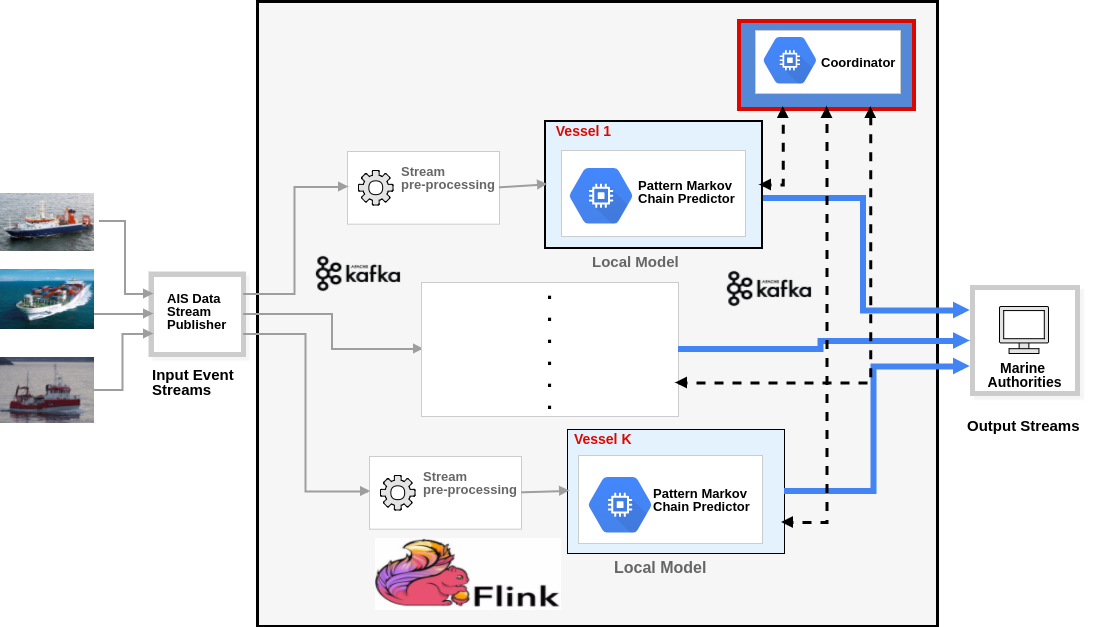
\includegraphics[width=0.9\textwidth]{figures/architecturedist.png}	
		
		%\hfill
		\caption{An Overview of Our Proposed System Architecture and  Implementation}  
		\label{fig:system_arch}
	\end{centering}
\end{figure} 

\subsection{Apache Flink}
 Apache Flink is an open source project that provides a large-scale, distributed and stateful stream processing platform \cite{carbone2015apache}. Flink is one of the recent and common big data processing frameworks, it employees data-stream processing model for streaming and batch data, the batch processing is treated as a special case of streaming applications (i.e., finite stream). The Flink's software stack includes the  $DataStream$ and $DataSet$ APIs for processing infinite and finite data, respectively. These two core APIs built on the top of the Flink's core distributed streaming dataflow engine. Additionally, Flink provides libraries such as Complex event processing for Flink (Flink-CEP), Machine Learning for Flink (FlinkML) and Flink Graph API (Gelly) \cite{carbone2015apache}.
 
 \par The main data abstractions of Flink are $DataStream$ and $DataSet$ that represent read-only collection of data elements. The list of elements is bounded (i.e., finite) in $DataSet$, while it is unbounded (i.e., infinite) in the case of $DataStream$. The Flink's core is a distributed streaming dataflow engine, with each
 Flink program is represented by a data-flow graph (i.e., directed acyclic graph - DAG) that executed by the Flink's engine \cite{carbone2015apache}. The data flow graphs are composed of stateful (state is maintained per partition), parallel operations and intermediate data stream partitions.
 
\subsection{Apache Kafka}

Apache Kafka is scalable, fault-tolerant and distributed streaming framework \footnote{\url{https://kafka.apache.org/}}. It allows to publish and subscribe to arbitrary data streams. Kafka manages the stream records in different categories (i.e., topics) that are partitioned and distributed over the Kafka servers. It provides the ability to publish a stream of records to one or more Kafka topic, to be consumed by applications that can subscribe to one or more topic to read data streams. The stream is distribute and balance between receivers within the same group for the sake of scalability.

\section{Experimental Evaluation}

\par In order to evaluate the performance of our proposed system, we will run it over synthetic data stream and large real-world data streams provided in the context of the datAcron project. Specifically, the event streams will be relevant to the maritime surveillance, for instance, the following are two different datasets to be used in generating simulated data streams : \begin{enumerate} 
	\item Raw Automatic Identification System (AIS) \footnote{AIS: \url{www.navcen.uscg.gov/?pageName=AISmain}} position messages of moving vessels.
	\item Critical points of trajectories of moving vessels (i.e., trajectory synopses) that derived form the raw AIS data as described in \citep{synopses1}.
\end{enumerate}




 .
\section{Work Plan}

We are planning to proceed working on this thesis according to a schedule (shown in Figure \ref{fig:work_plan}) as follows: in the first month we will study related work and algorithms in depth. Then, in the second and third month we will implement the system on top of
datAcron project and run experiments to evaluate the our system over the different data sources, and start the theoretical analysis. Then, by the fourth month we will have completed system's implementation and initial evaluation. While the fifth and sixth months will be dedicated for carrying out extensive experiments and finish  writing the thesis's report.

\begin{figure}[!ht]
	\begin{centering}
		
			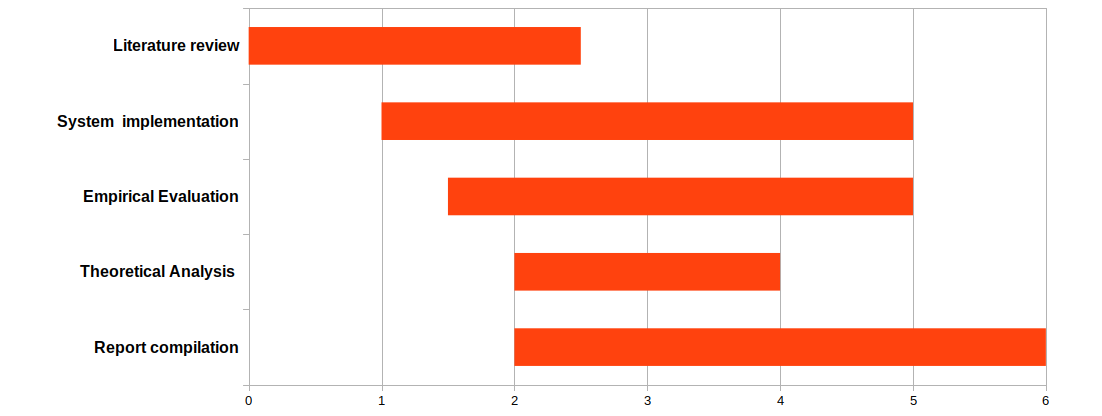
\includegraphics[width=0.9\textwidth]{figures/plan.png}	
	
		%\hfill
		\caption{Thesis work plan.}  
			\label{fig:work_plan}
	\end{centering}
\end{figure}

%
\section{extra}
Data Mining and Knowledge Discovery
Springer (www.springer.com/10618)

Final Call for Papers
Special Issue on "Data Mining for Geosciences"
-------------------------------------------------------------------------------

Modern geosciences have to deal with large quantities and a wide variety of data, including 2-D, 3-D and 4-D seismic surveys, well logs generated by sensors, detailed lithological records, satellite images and meteorological records. These data serve important industries, such as the exploration of mineral deposits and the production of energy (Oil and Gas, Geothermal, Wind, Hydroelectric), are important in the study of the earth crust to reduce the impact of earthquakes, in land use planning, and have a fundamental role in sustainability. In particular, the process of exploring and exploiting Oil and Gas (OG) generates a lot of data that can bring more efficiency to the industry. The opportunities for using data mining techniques in the "digital oil-field" remain largely unexplored or uncharted.The purpose of this special issue is to be a breaking-edge showcase for applications and developments of data mining and knowledge discovery in the area of the geosciences with a special focus in the oil and gas exploration. Researchers are invited to submit original papers presenting novel data mining methodologies or applications to the geosciences, including but not limited to the following topics:

\* Oil and gas exploration and production
* Mineral deposit/reservoir identification and characterization
* Exploration of well-log data
* Earth crust analysis and understanding
* Sensor data exploration
* Remote sensing
* Novel data mining problems in the geosciences
* Visualization of big data in the geosciences
* Geoscience data fusion for enhancing data mining solutions
* Data streams analysis in geoscience
* Feature extraction and data transformation from geoscientific data



\textbf{
. A maximum likelihood estimate of the Markov transition matrix is constructed by joint unbiasing of the transition counts from multiple umbrella-sampling simulations along discretized reaction coordinates}


%{\centering  
%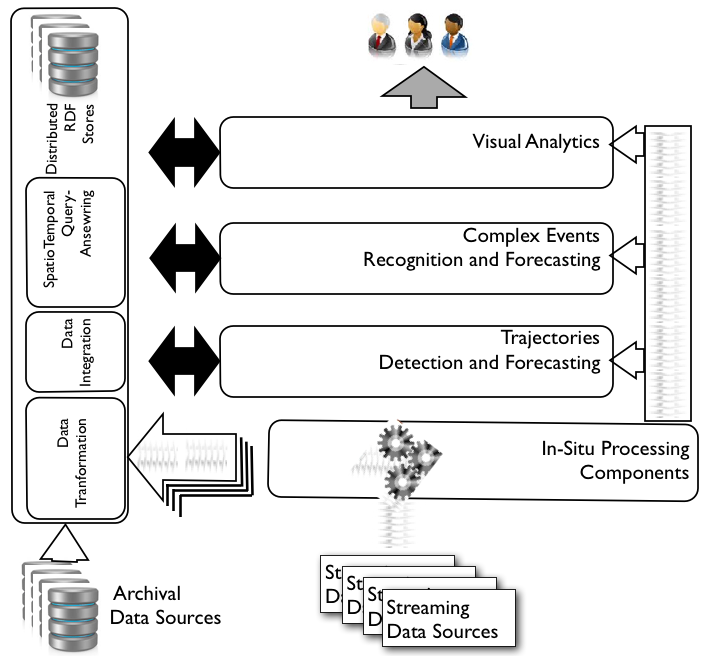
\includegraphics[width=4.972in,height=3.5693in]{figures/datACRONDXYTemplate201512162-img002.png}
% \par}
%
%\captionof{figure}{datACRON Overall Architecture }
%
%
%
%\begin{flushleft}
%\begin{tabular}{m{0.48in}|m{3.29in}|m{1.89in}c|}
%\hline
%\rowcolor{datacroninner}
%{\bfseries\color{white}lala}&{\bfseries\color{white} Bla} &{\bfseries\color{white} bla}\\\hline
%1 &~ &~\\\hline
%2 &~ &~\\\hline
%\end{tabular}
%\end{flushleft}


\clearpage
%\nocite{*}
%\bibliographystyle{plain-annote}
%\bibliographystyle{plainnat}
 \bibliographystyle{agsm} 
\bibliography{myrefs}
\end{document}



